\documentclass[12pt,hyperref,a4paper,UTF8]{ctexart}
\usepackage{HDUReport}
\usepackage{listings}
\usepackage{xcolor}
\usepackage{graphicx}
\usepackage{setspace}
\usepackage{float}
\setstretch{1.5} % 设置全局行距为1.5倍

\usepackage{enumitem} % 载入enumitem包以便自定义列表环境
\setlist[itemize]{itemsep=0pt, parsep=0pt} % 设置itemize环境的项目间距和段落间距

\setmainfont{Times New Roman} % 英文正文为Times New Roman


\usepackage{tikz}
\usetikzlibrary{shapes.geometric, arrows}
\usetikzlibrary{positioning, arrows.meta}
\usetikzlibrary{calc}
%封面页设置
{   
    %标题
    \title{ 
        \vspace{1cm}
        \heiti \Huge \textbf{《单片机原理及应用》作业报告} \par
        \vspace{1cm} 
        \heiti \Large {\underline{实验报告2第二部分:单灯闪烁}   } 
        \vspace{3cm}
    
    }

    \author{
        \vspace{0.5cm}
        \kaishu\Large 学院\ \dlmu[9cm]{卓越学院} \\ %学院
        \vspace{0.5cm}
        \kaishu\Large 学号\ \dlmu[9cm]{23040447} \\ %班级
        \vspace{0.5cm}
        \kaishu\Large 姓名\ \dlmu[9cm]{陈文轩} \qquad  \\ %学号
        \vspace{0.5cm}
        \kaishu\Large 专业\ \dlmu[9cm]{智能硬件与系统(电子信息工程)} \qquad \\ %姓名 
    }
        
    \date{\today} % 默认为今天的日期,可以注释掉不显示日期
}
%%------------------------document环境开始------------------------%%
\begin{document}

%%-----------------------封面--------------------%%
\cover
\thispagestyle{empty} % 首页不显示页码
%%------------------摘要-------------%%
%\newpage
%\begin{abstract}




%\end{abstract}

%\thispagestyle{empty} % 首页不显示页码

%%--------------------------目录页------------------------%%
% \newpage
% \tableofcontents
% \thispagestyle{empty} % 目录不显示页码

%%------------------------正文页从这里开始-------------------%
\newpage
\setcounter{page}{1} % 让页码从正文开始编号

%%可选择这里也放一个标题
%\begin{center}
%    \title{ \Huge \textbf{{标题}}}
%\end{center}

\section{原题目}

\textbf{通过软硬件设计实现1个LED灯单灯闪烁,灯亮时间自选。用Proteus软件仿真。用C语言编程。}

\section{实验程序}
\begin{lstlisting}[language=C, caption={数据迁移实验程序}]
#include <reg51.h>  // 51单片机头文件

sbit LED = P1^0;    // LED连接P1.0

// 定时器初始化(方式1,16位定时器)
void Timer0_Init() {
    TMOD |= 0x01;    // 定时器0,模式1
    TH0 = 0x3C;      // 定时50ms(12MHz晶振)
    TL0 = 0xB0;      //初值 = 65536 - 50000 = 15536 = 0x3CB0 
                        //即计数50000次,就是50ms=50000*1us
    ET0 = 1;         // 允许定时器0中断
    EA = 1;          // 全局中断使能
    TR0 = 1;         // 启动定时器0
}

// 定时器0中断服务程序
void Timer0_ISR() interrupt 1 {
    static unsigned int count = 0;
    TH0 = 0x3C;      // 重新装载初值 手动赋值装载
    TL0 = 0xB0;
    count++;
    if (count >= 20) {  // 20*50ms = 1s
        count = 0;
        LED = ~LED;     // LED状态取反
    }
}

void main() {
    LED = 0;          // 初始状态(LED灭)
    Timer0_Init();    // 初始化定时器
    while (1);        // 主循环(中断驱动)
}
    
\end{lstlisting}

\section{实验效果}

\begin{figure}[H] % [H] 表示强制当前位置插入
    \centering
    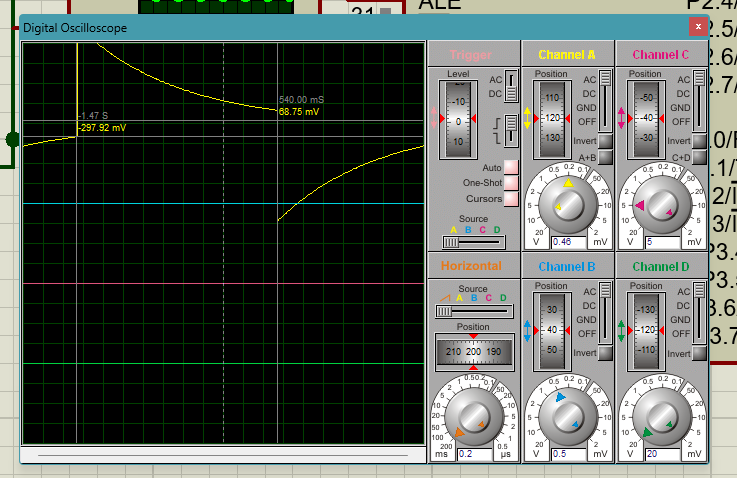
\includegraphics[width=0.8\textwidth]{figures/201.png} % 调整宽度为文本宽度的 80%
    \caption{Proteus示波器效果,脉宽手动测量约1S} % 图片标题
    \label{fig:example} % 图片标签,用于引用
\end{figure}

\begin{figure}[H] % [H] 表示强制当前位置插入
    \centering
    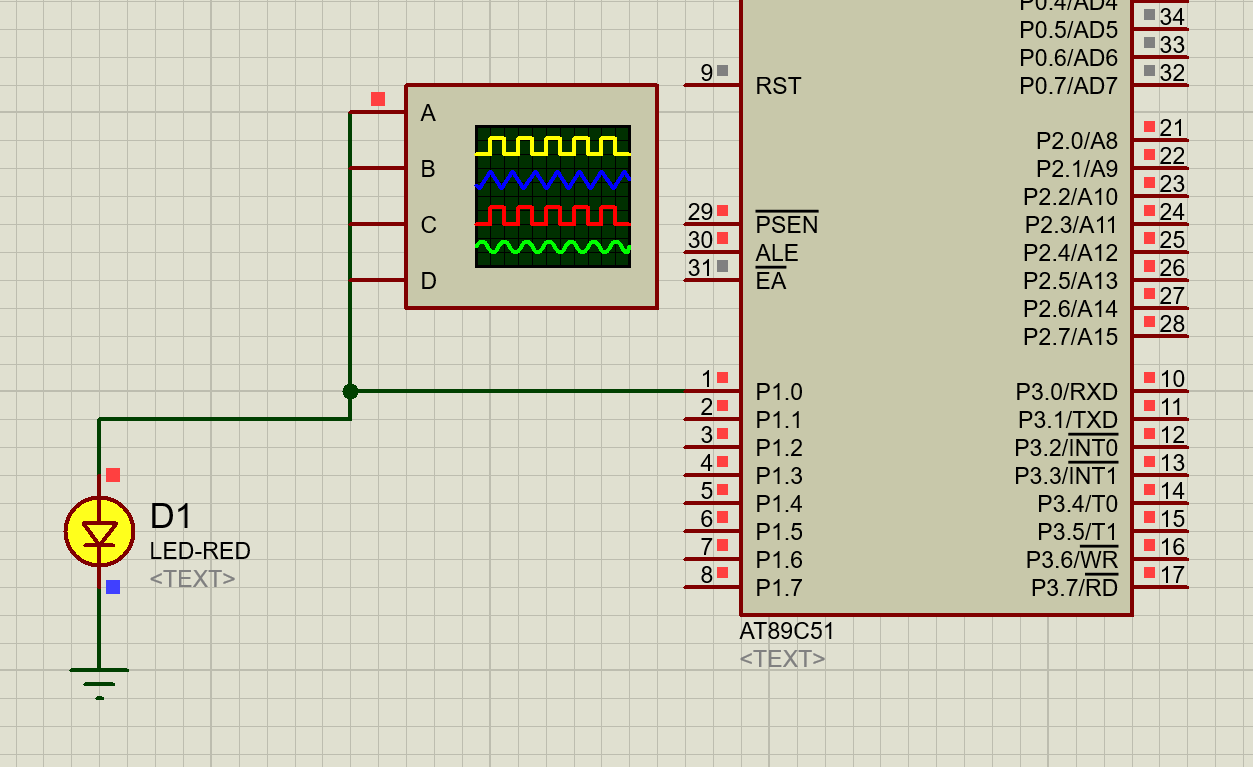
\includegraphics[width=0.8\textwidth]{figures/202.png} % 调整宽度为文本宽度的 80%
    \caption{Proteus灯亮效果} % 图片标题
    \label{fig:example} % 图片标签,用于引用
\end{figure}

\begin{figure}[H] % [H] 表示强制当前位置插入
    \centering
    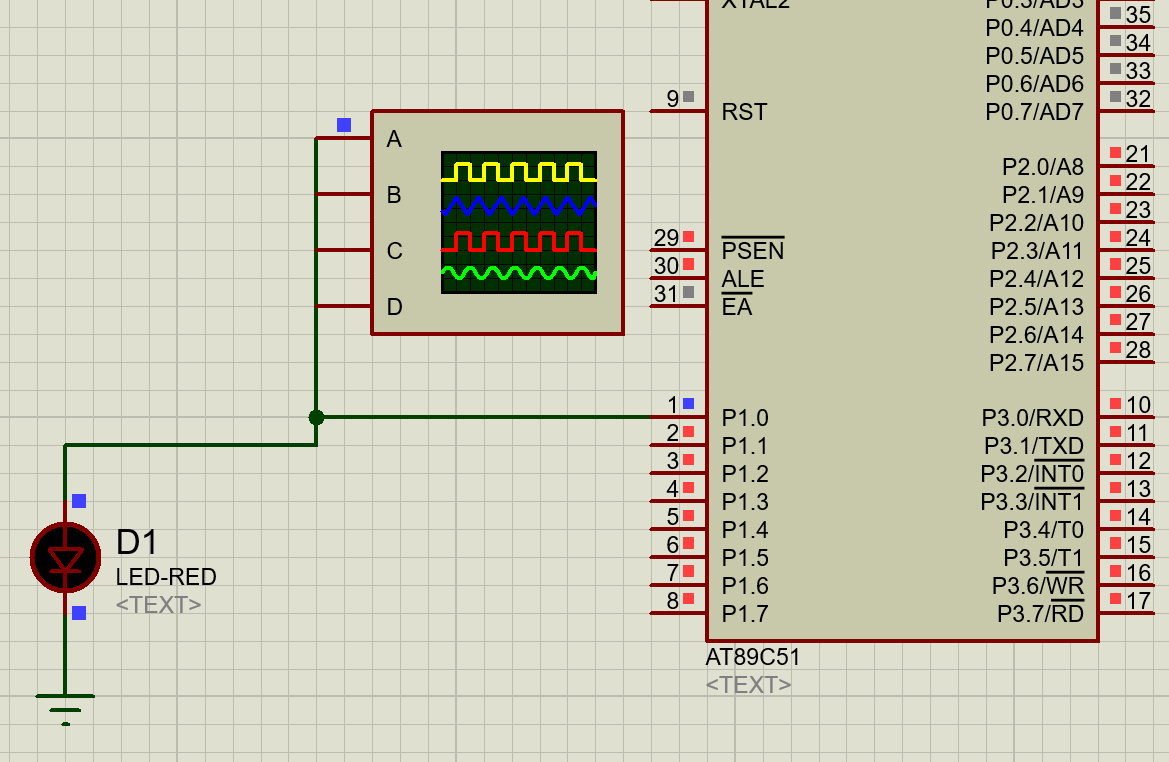
\includegraphics[width=0.8\textwidth]{figures/203.png} % 调整宽度为文本宽度的 80%
    \caption{Proteus灯灭效果} % 图片标题
    \label{fig:example} % 图片标签,用于引用
\end{figure}


\section{流程图}

\begin{figure}[H]
    \centering
    \begin{tikzpicture}[
        node distance=1.5cm,
        startstop/.style={rectangle, rounded corners, minimum width=3cm, minimum height=1cm, text centered, draw=black, fill=red!30},
        process/.style={rectangle, minimum width=3cm, minimum height=1cm, text centered, draw=black, fill=blue!30},
        decision/.style={diamond, aspect=1.8, minimum width=2.5cm, minimum height=1.8cm, text centered, draw=black, fill=green!30},
        arrow/.style={thick, -Stealth}
    ]

        % ===== 主流程 =====
        \node (start) [startstop] {程序开始};
        \node (initLED) [process, below=of start] {初始化 LED};
        \node (initTimer) [process, below=of initLED] {初始化定时器};
        \node (loop) [process, below=of initTimer] {主循环等待中断};
        
        % ===== 中断处理 =====
        \node (interrupt) [decision, right=5cm of loop] {定时器中断触发?};
        \node (reload) [process, below=2cm of interrupt] {重装定时器初值};
        \node (countCheck) [decision, below=2cm of reload] {计数 $\geq$ 20?};
        \node (toggleLED) [process, left=3cm of countCheck] {LED 状态取反};
        \node (resetCount) [process, below=1cm of toggleLED] {计数器清零};

        % ===== 绝对坐标关键点定义 =====
        \coordinate (loopExit) at ($(loop.east)+(2cm,0)$);
        \coordinate (interruptReturn) at ($(interrupt.east)+(2cm,0)$);
        \coordinate (loopReturnTop) at ($(loop.north east)+(0,0.5cm)$);
        \coordinate (resetReturn) at ($(resetCount.west)-(2cm,0)$);

        % ===== 优化后的箭头路径 =====
        % 主流程
        \draw [arrow] (start) -- (initLED);
        \draw [arrow] (initLED) -- (initTimer);
        \draw [arrow] (initTimer) -- (loop);
        
        % 中断检测(完全重构路径)
        \draw [arrow] (loop.east) -- (loopExit) -- (interrupt.west);
        \draw [arrow] (interrupt.south) -- node[right] {是} (reload.north);
        
        % 中断"否"路径(关键优化)
        \draw [arrow] (interrupt.east) -- (interruptReturn) 
            -- ++(0,1.2cm) node[above left] {否} 
            -| (loopReturnTop) -- (loop.north east);
        
        % 中断处理
        \draw [arrow] (reload.south) -- (countCheck.north);
        \draw [arrow] (countCheck.west) -- node[above] {是} (toggleLED.east);
        \draw [arrow] (toggleLED.south) -- (resetCount.north);
        
        % 返回路径(双重避让)
        \draw [arrow] (resetCount.west) -- (resetReturn) 
            |- ($(loop.west)-(0,0.3cm)$) -- (loop.west);
        \draw [arrow] (countCheck.east) -- ++(1.5cm,0) node[above right] {否} 
            |- ($(reload.east)+(0,-0.5cm)$) -- (reload.east);

    \end{tikzpicture}
    \caption{单灯闪烁程序流程图}
    \label{fig:ultimate_flowchart}
\end{figure}



\section{实验体会}

实验通过定时器模式1下,对于TL0,TX0定时器计数器的手动重装载,实现了特定时间的定时控制,以此控制灯亮脉宽。
这让我更加熟悉了定时器的使用,指定寄存器的赋值等操作,对于51单片机的学习很有帮助。




\end{document}